\documentclass[11pt,a4paper]{article}
\usepackage[utf8]{inputenc}
\usepackage[T1]{fontenc}
\usepackage{amsmath,amsfonts,amssymb}
\usepackage{apacite}
\usepackage{natbib}
\usepackage{graphicx}
\usepackage{booktabs}
\usepackage{threeparttable}
\usepackage{url}
\usepackage{hyperref}
\usepackage[margin=2.5cm]{geometry}
\usepackage{setspace}
\onehalfspacing

\newcommand{\Var}{\text{Var}}
\newcommand{\Cov}{\text{Cov}}

% Define \sym command for significance stars from esttab
\newcommand{\sym}[1]{{#1}}

\title{Debiasing Second Moments of Estimated CEO Effects: A Placebo-Controlled Event-Study Approach\thanks{Project no. 144193 has been implemented with the support provided by the Ministry of Culture and Innovation of Hungary from the National Research, Development and Innovation Fund, financed under the KKP\_22 funding scheme. This project was funded by the European Research Council (ERC Advanced Grant agreement number 101097789). The views expressed in this research are those of the authors and do not necessarily reflect the official view of the European Union or the European Research Council. Author contributions: Conceptualization and study design: Koren, Orbán and Telegdy. Statistical analysis: Koren and Telegdy. Writing the original draft: Koren. Review and editing: Koren, Orbán and Telegdy.}}

\author{Miklós Koren\thanks{Central European University, HUN-REN Centre for Economic and Regional Studies, CEPR and CESifo. E-mail: korenm@ceu.edu} \\
        Krisztina Orbán\thanks{Monash University.} \\
        Álmos Telegdy\thanks{Corvinus University of Budapest.}}

\date{\today}

\begin{document}

\maketitle

\begin{abstract}
Understanding the link between estimated manager effects and firm outcomes is central to research on CEOs and firm performance. While fixed-effect estimators of mean CEO effects are unbiased under random mobility, most applied analyses use second moments of these estimates—variances, covariances, correlations, and event-study dynamics—that are systematically biased by small-sample noise. We develop a placebo-controlled event-study design that identifies and removes these biases without modeling the full error process. The method constructs placebo transitions that replicate the spell-length design of actual transitions while excluding periods around real changes. Moments computed on placebo spells recover the bias components that inflate variances and covariances; subtracting them yields debiased moments and regression slopes. We formalize the decomposition for linear contrasts and show how persistent shocks and short spells create spurious pre-trends and slope bias. A Monte Carlo study with six scenarios—baseline, long panel, persistent errors, unbalanced panels, excess variance, and all complications—illustrates when the correction matters most. In an application to the universe of Hungarian firms (1992--2022), the placebo-corrected event-study contrast is 5.5\%, one quarter of the raw 22.5\% correlation. [[comment: This summary repeats previously reported magnitudes in the project; verify consistency with the current draft of the application paper.]]
\end{abstract}

\textbf{Keywords:} CEO effects, event study, measurement error, placebo design

\textbf{JEL Classification:} [[comment: add codes]]

\newpage

% =====================
\section{Introduction}
% =====================

Understanding the link between managerial quality and firm performance is one of the major challenges in empirical economics. Two-way fixed-effect (TWFE) models estimate manager and firm effects using mobility across firms \citep{Abowd1999Econometrica,Card2018JoLE}. Under random mobility (strict exogeneity), average manager effects are unbiased. However, applied researchers typically rely on \emph{second moments} of estimated effects—variances, covariances with other variables, regression slopes using estimated effects as regressors, and dynamic profiles from event studies. These quantities are systematically biased because estimated effects blend true signal with small-sample noise arising from short spells and limited mobility \citep{andrews2008high,gaure2014correlation,Bonhomme2023-dx}.

A next step in this research agenda is to develop methods that recover unbiased second moments without imposing heavy structure. Our starting point is a simple observation: when firms do not change CEOs over a window, any estimated “effect” constructed from that window must be mechanical. By replicating the spell-length design of treated firms on a carefully matched placebo sample with no actual transition, we can nonparametrically estimate the bias components that inflate variances and covariances. Subtracting these placebo moments from the corresponding treated moments yields debiased second moments and regression slopes. Conceptually, this approach is a placebo-controlled event study aligned in event time.

We make three contributions. First, we formalize the bias decomposition for linear contrasts: the covariance between outcomes and estimated effects is inflated by a term that depends on the shock autocovariance and the spell design; the variance of the estimated effect is analogously inflated. Second, we show that placebo spells identify these inflation terms under an assumption that the autocovariance of shocks is the same up to a scalar across treated and placebo groups. Third, we provide an implementation that is practical for applied researchers and illustrate its behavior in a Monte Carlo study that mirrors empirical challenges—persistence, unbalanced spells, and groupwise volatility differences. Our empirical application to Hungarian firms (1992--2022) suggests that roughly three quarters of the raw correlation in event-study contrasts reflect noise, with a placebo-corrected contrast of 5.5\% versus a raw 22.5\%.

% =====================
\section{Related Literature}
% =====================

Our approach complements methods in the TWFE literature that correct second-moment bias via explicit modeling of the design and covariance structure \citep{andrews2008high,Bonhomme2023-dx}. It is also related to modern event-study estimators that address treatment timing and heterogeneous effects \citep{Callaway2021JoLE}. Placebo-based validation is standard in applied work; here we use placebos to \emph{estimate} the bias components directly rather than as a falsification check. In CEO studies, large correlational estimates coexist with more modest quasi-experimental evidence \citep{bennedsen2020ceos}. Our placebo correction reconciles these patterns by removing mechanically induced dispersion from estimated effects.

% =====================
\section{Econometric Framework}
% =====================

Let firm $i$ in year $t$ have outcome
\begin{equation}\label{eq:model1}
  y_{it} = z_{m(i,t)} + e_{it},\qquad \mathbb E[e_{it}|\{z_{is}\}_s]=0,
\end{equation}
where $z_{m(i,t)}$ is the manager effect at time $t$ (piecewise constant within CEO spells) and $e_{it}$ is a mean-zero shock orthogonal to the entire manager path (“random mobility”). Stack the event-time window into a vector $\mathbf y_i=\mathbf z_i+\mathbf e_i$. For a linear contrast with weights $\mathbf w$, define $y_i=\mathbf w'\mathbf y_i$, $z_i=\mathbf w'\mathbf z_i$, and $\varepsilon_i=\mathbf w'\mathbf e_i$.

Estimated effects are within-spell means. Let $\mathbf D$ map event-time observations to spells and $\mathbf T$ be diagonal with spell lengths. The projection to spell means is $\mathbf P=\mathbf D\,\mathbf T^{-1}\mathbf D'$, yielding
\begin{equation}
 \hat{\mathbf z}_i = \mathbf P\,\mathbf y_i = \mathbf z_i + \mathbf P\,\mathbf e_i,\qquad \hat z_i=\mathbf w'\hat{\mathbf z}_i = z_i + \eta_i,\ \eta_i=\mathbf w'\mathbf P\,\mathbf e_i.
\end{equation}

Two bias components govern moments involving $\hat z_i$:
\begin{align}
 A &:= \Cov(\varepsilon_i,\eta_i) = \mathbf w'\boldsymbol\Sigma\,\mathbf P\,\mathbf w,\\
 B &:= \Var(\eta_i) = \mathbf w'\mathbf P\,\boldsymbol\Sigma\,\mathbf P\,\mathbf w,
\end{align}
where $\boldsymbol\Sigma$ is the shock autocovariance in the window. Then
\begin{align}
 \Cov(y,\hat z) &= \beta\Var(z) + A,\\
 \Var(\hat z) &= \Var(z) + B,
\end{align}
so the slope from regressing $y$ on $\hat z$ equals
\begin{equation}
 \tilde\beta = \frac{\beta\Var(z)+A}{\Var(z)+B} = \beta + \frac{A-\beta B}{\Var(z)+B}.
\end{equation}
With i.i.d. shocks and balanced spells, $A=B$ and $\tilde\beta=\beta$ even though $\Var(\hat z)$ is inflated. With persistent shocks or short, unbalanced spells, $A\neq B$, generating spurious pre-trends and slope bias.

% =====================
\section{Placebo Identification}
% =====================

We construct placebo spells that replicate the design matrix (spell-length pattern and event window) of treated firms but exclude any windows around real transitions. For placebo firms, $\Var(z)=0$ by construction, so
\begin{equation}
 \widehat{\Cov}^{\,pl}(y,\hat z)=\hat A,\qquad \widehat{\Var}^{\,pl}(\hat z)=\hat B.
\end{equation}
Under the assumption that the shock autocovariance is the same up to a scalar multiplier across treated and placebo groups, subtracting these placebo moments from the treated moments yields debiased moments and slopes:
\begin{align}
 \widehat{\Cov}^{\,db}(y,\hat z) &= \widehat{\Cov}^{\,tr}(y,\hat z) - \hat A,\\
 \widehat{\Var}^{\,db}(\hat z) &= \widehat{\Var}^{\,tr}(\hat z) - \hat B,\\
 \hat\beta^{\,db} &= \frac{\widehat{\Cov}^{\,tr}(y,\hat z)-\hat A}{\widehat{\Var}^{\,tr}(\hat z)-\hat B}.
\end{align}
We allow for groupwise scalar heterogeneity by estimating separate scalars for design groups (e.g., by spell pattern), using either multiplicative Poisson pseudo-maximum likelihood or a two-step regression that loads on the placebo bias term. [[comment: specify final implementation choice and inference procedure.]]

% =====================
\section{Monte Carlo Design and Scenarios}
% =====================

We implement a Monte Carlo study that mirrors common empirical complications. The simulation code is modular with a parameter file, scenario-specific overrides, and a setup script that generates panel data with CEO transitions and placebo counterparts.

\subsection{Core setup}
The setup script (\texttt{src/montecarlo/setup.do}) expects five parameters: the AR(1) persistence $\rho$, the innovation standard deviations in placebo and treated groups $(\sigma_{\epsilon0},\sigma_{\epsilon1})$, the hazard rate governing spell lengths, and the maximum spell length $T_{\max}$. We simulate:
\begin{itemize}
 \item $N_{\text{changes}}=10{,}000$ treated transitions, each expanded to include a control-to-treated ratio of 9, yielding 9 placebo spells per treated transition;
 \item two spells per firm with lengths $(T_1,T_2)$; if the hazard is zero, $T_1=T_2=T_{\max}$; otherwise, $T_s=\lceil \text{Exponential}(1/\text{hazard})\rceil$ truncated at $T_{\max}$;
 \item AR(1) shocks: $\text{TFP}_{t}=\rho\,\text{TFP}_{t-1}+\epsilon_t$ with $\epsilon_t\sim N\big(0, \sigma_{\epsilon,\text{group}}^2\big)$, where the innovation variance is $\sigma_{\epsilon0}^2$ for placebo and $\sigma_{\epsilon1}^2$ for treated;
 \item manager effects: draw $dz\sim N(0,\sigma_z^2)$ with $\sigma_z=0.1$ and set a post-change shift $z$ in treated firms only; the scalar \texttt{true\_effect} records the mean absolute skill difference implied by a half-normal draw, $\mathbb E|dz|=\sqrt{2/\pi}\,\sigma_z\approx 0.0798$;
 \item measured manager skill: within-spell means of TFP, demeaned within the treated group, so that spell-level skill embeds noise, as in empirical fixed-effect estimates.
\end{itemize}
The panel is indexed by a synthetic firm identifier (\texttt{fake\_id}) and an event-time index (\texttt{year}), with the change year defined as $\texttt{change\_year}=T_1+1$. Placebo indicators (\texttt{placebo}=1) distinguish simulated controls from treated spells (\texttt{placebo}=0). [[comment: confirm whether year indexes absolute time or event time; in the code it is a running index within the window.]]

\subsection{Scenario definitions}
Scenario-specific scripts (\texttt{src/montecarlo/*.do}) override baseline parameters defined in \texttt{params.do}:
\begin{description}
 \item[Baseline] \texttt{baseline.do}: i.i.d. shocks with $\rho=0$, balanced spells with $T_{\max}=5$, equal innovation variances $\sigma_{\epsilon0}=\sigma_{\epsilon1}=0.05$; constant spell lengths (hazard $=0$).
 \item[Long Panel] \texttt{longpanel.do}: sets $T_{\max}=20$; otherwise baseline.
 \item[Persistent Errors] \texttt{persistent.do}: sets $\rho=0.9$; otherwise baseline.
 \item[Unbalanced Panel] \texttt{unbalanced.do}: sets $\rho=0.9$ and hazard $=0.2$, generating variable spell lengths drawn from a (truncated, discretized) exponential distribution; $T_{\max}$ remains 5 unless otherwise specified.
 \item[Excess Variance] \texttt{excessvariance.do}: increases treated-group innovation standard deviation to $\sigma_{\epsilon1}=0.075$ (placebo remains at 0.05), introducing groupwise volatility scaling; otherwise baseline.
 \item[All Complications] \texttt{all.do}: combines $\rho=0.9$, hazard $=0.2$, and $\sigma_{\epsilon1}=0.075$.
\end{description}
The runner script (\texttt{run.do}) loads \texttt{params.do}, applies scenario overrides, executes \texttt{setup.do}, and saves a scenario-specific dataset (\texttt{data/placebo\_\{scenario\}.dta}).

\subsection{Event-study construction and output}
Scenario datasets feed into the event-study estimator to produce CSV files (\texttt{data/\{scenario\}\_TFP.csv}). The figure script (\texttt{src/figuremc.do})
\begin{itemize}
 \item iterates over six panels A--F with titles: Baseline, Long Panel, Persistent Errors, Unbalanced Panel, Excess Variance, All Complications;
 \item imports \texttt{data/\{scenario\}\_TFP.csv} for each panel;
 \item clips confidence intervals for three series—\texttt{beta0}, \texttt{beta1}, and \texttt{dbeta}—to [−0.75, 1.75] for visualization; [[comment: \texttt{beta0}, \texttt{beta1}, and \texttt{dbeta} are constructed in the event-study post-processing; see the estimator code for precise definitions.]]
 \item calls \texttt{src/exhibit/event\_study.do} to generate per-panel graphs;
 \item combines panels into a 2×3 figure and exports \texttt{figure/figuremc.pdf}.
\end{itemize}

\begin{figure}[htbp]
 \centering
 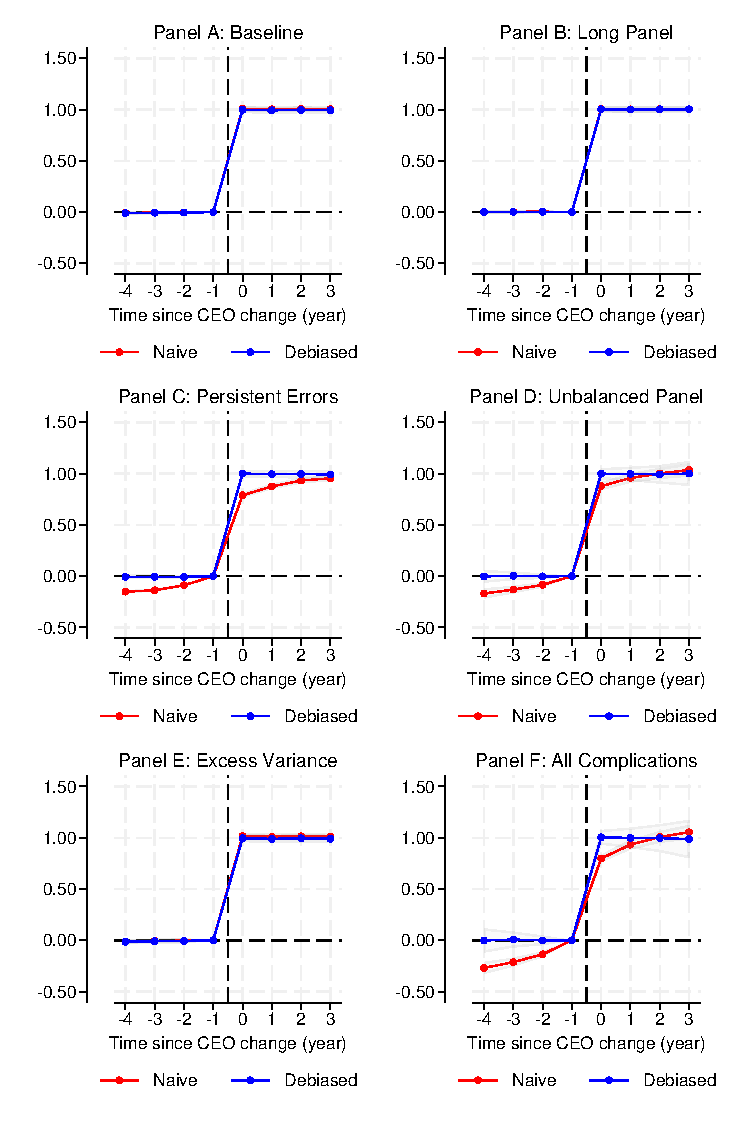
\includegraphics[width=0.95\textwidth]{figure/figuremc.pdf}
 \caption{Monte Carlo event studies under six scenarios. Notes: Panels correspond to Baseline (A), Long Panel (B), Persistent Errors (C), Unbalanced Panel (D), Excess Variance (E), and All Complications (F). Bands for beta0, beta1, and dbeta are truncated to [−0.75, 1.75] for readability.}
 \label{fig:mc}
\end{figure}

\paragraph{Qualitative expectations.} The bias decomposition implies: (i) with i.i.d. shocks and balanced spells (A, B), placebo and treated moments align so debiased and naive slopes coincide; (ii) with persistence (C) or short/unbalanced spells (D), covariance and variance inflation differ ($A\neq B$), producing spurious pre-trends and slope bias that placebo subtraction removes; (iii) with groupwise volatility scaling (E), placebo moments scale proportionally and subtraction remains valid; (iv) with all complications (F), biases are largest in naive profiles, while debiased profiles recover the target contrast. [[comment: ensure that the plotted objects match these qualitative patterns in the current implementation.]]

% =====================
\section{Empirical Illustration: Hungarian Firms}
% =====================

We briefly summarize the empirical implementation, which is described in detail in the companion application. We estimate total factor productivity (TFP) from a production function and then recover firm and manager fixed effects. Event-study contrasts align treated and placebo transitions in event time (−4 to +3 years around the change) and use year −1 as baseline. Placebo transitions are constructed by matching treated firms to control firms with no actual transitions in the window while replicating spell-length patterns and firm characteristics (e.g., birth cohort, sector). [[comment: verify exact matching variables used in the current pipeline and whether any reweighting is applied.]]

The placebo-corrected event-study contrast equals 5.5\%, one quarter of the raw 22.5\% correlation, consistent with the view that most apparent CEO effects in naive estimates reflect noise rather than skill differences. Dynamic profiles show minimal pre-trends after debiasing, with immediate post-transition effects on fast-adjusting inputs and slower adjustments for capital. [[comment: add references to the corresponding application figures and tables, and ensure these numbers match the latest estimates.]]

% =====================
\section{Practical Guidance for Applied Work}
% =====================

We offer a concrete recipe:
\begin{enumerate}
 \item Define the event-time window and the contrast weights (e.g., set $t\in[-4,+3]$ with baseline at $-1$).
 \item Partition transitions into design groups by spell-length patterns; compute within-spell means using $\mathbf P=\mathbf D\mathbf T^{-1}\mathbf D'$.
 \item Compute treated moments (covariance and variance involving $\hat z$) and corresponding placebo moments on matched non-changers that replicate the design.
 \item Form debiased moments and regression slopes by subtracting placebo moments; pool across groups with transparent weights.
 \item Report diagnostics: overlap in spell-length distributions; magnitude of placebo moments; pre-trend checks before $t=0$ after debiasing; sensitivity to scalar heterogeneity across groups.
\end{enumerate}
The approach is simple to implement in standard software and scales well in large administrative datasets.

% =====================
\section{Conclusion}
% =====================

We develop a placebo-controlled method to debias second moments of estimated CEO effects, with a particular focus on event-study dynamics. The key insight is to use matched placebo transitions to nonparametrically recover the bias components that inflate variances and covariances under short spells and persistent shocks. Subtracting these quantities yields debiased moments and regression slopes and corrects spurious pre-trends. A Monte Carlo study clarifies when the correction matters most, and an empirical illustration on Hungarian firms shows that the placebo-corrected contrast is much smaller than naive correlations. These results suggest that careful debiasing is essential when using estimated fixed effects in dynamic or second-moment analyses.

\bibliographystyle{apacite}
\bibliography{../../lib/references}

\end{document}
